% Provenance (never printed): see sources/outline_sources.md (Year 1: decay systems K-Ar,
% Rb-Sr, U-Pb and radiocarbon; closure temperature; dating sedimentary sequences with
% volcanic ashes; calibrating the scale). Exercise and problem values in the Book 3
% scratch calculator calc/ch25.py; figures from figdata/bachelor-1/decay_curves.py,
% isochron.py and radiocarbon.py (IntCal20, dataset bachelor-1-intcal20).
% The decay law, half-life and decay constant belong to the physics series (recalled);
% the closed system and the isochron of minerals are Book 2's (g12 age-of-the-earth),
% re-founded here with whole-rock samples and least squares. The concordia diagram and
% thermochronology are the Year 3 volume's: prose pointers only. Mass spectrometry is
% the chemistry series' (recalled). The isochron figure uses an invented rhyolite so that
% the Varden granite of the problem is not solved in the course.
\chapter{Métodos de datação radiométrica}\label{ch:b1:radiometric-methods}

Em 2001 uma equipe que trabalhava com grãos detríticos de zircão das Jack Hills, na Austrália
Ocidental, relatou um que havia cristalizado há \num[uncertainty-mode=separate]{4404 \pm 8} milhões
de anos. Trabalhos posteriores confirmaram a idade desses grãos: são o material mais antigo já
formado na Terra, de qualquer tipo, e mostram que uma \omterm{def:b1:layered-earth:layers}{crosta} havia se formado em cerca de 160
milhões de anos do nascimento do Sistema Solar. No outro extremo da escala, idades argônio
situaram a extinção no fim do Cretáceo, há \qty{66.00}{\Ma}, a menos de \num{32000} anos do
impacto que se pensa tê-la causado. Os dois números vêm da contagem de átomos: um pai radioativo
que decai a uma taxa conhecida, uma filha que se acumula. Este capítulo explica como tais
relógios são lidos, por que cada um data um evento diferente, e como eles penduram a escala de
\cref{ch:b1:stratigraphic-scale} em uma escala de anos.
% ledger: wilde01:4404, uw14:jack-hills, ics:base.Paleogene, renne:kpg

\begin{omfigure}
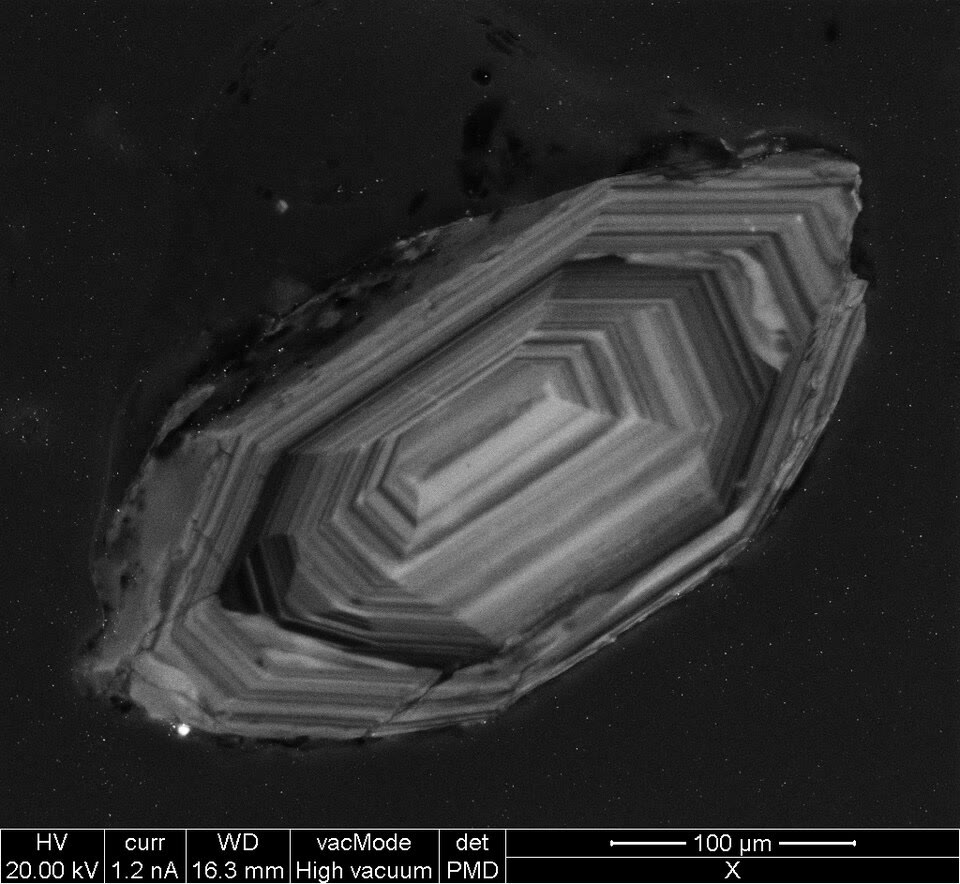
\includegraphics[width=0.5\linewidth]{images/book3/b1-zircon-cl.jpg}

{\small Um grão de zircão, de cerca de um terço de milímetro de comprimento, fotografado pela luz
que emite sob o feixe de elétrons de um microscópio eletrônico de varredura
(catodoluminescência). As faixas que seguem as faces do cristal são zonas de composição
ligeiramente diferente, depositadas uma após a outra à medida que ele crescia. Este grão foi
extraído de um arenito, então é mais antigo que o arenito: ele data a rocha de onde foi erodido.
(Emmanuel Roquette, CC~BY-SA~4.0, via Wikimedia Commons.)}
\label{fig:b1:radiometric-methods:zircon}
\end{omfigure}
% ledger: commons:zircon-cl

\begin{recall}
Os livros de física descrevem a desintegração radioativa: os núcleos de um isótopo radioativo
decaem ao acaso, independentemente da temperatura e da pressão, de modo que o número $N$ que
resta após um tempo $t$ segue $N = N_0\,e^{-\lambda t}$, em que $\lambda$ é a constante de
decaimento; a meia-vida é $T = \ln 2/\lambda$. Isótopos de um elemento têm o mesmo número de
prótons e números diferentes de nêutrons; os livros de química descrevem o espectrômetro de
massa, que separa íons por massa. No Livro~2, 12º ano, uma rocha ou \omterm{def:b1:rock-forming-minerals:mineral}{mineral} que não trocou
átomos-pai ou filha com seu entorno é um sistema fechado, e os \omterm{def:b1:rock-forming-minerals:mineral}{minerais} do granito de Varden,
plotados em uma \omterm{def:b1:radiometric-methods:isochron}{isócrona} rubídio--estrôncio, deram uma idade de 310 milhões de anos. Biotita,
muscovita e hornblenda são as \omterm{def:b1:rock-forming-minerals:groups}{micas} e o \omterm{def:b1:rock-forming-minerals:groups}{anfibólio} de \cref{def:b1:rock-forming-minerals:groups}.
Uma idade entre dois níveis datados pode ser interpolada
(\cref{prop:b1:stratigraphic-scale:interpolation}).
\end{recall}
% ledger: tulane:radiometric, villa22:rb87

\section{Sistemas de decaimento}\label{sec:b1:radiometric-methods:systems}

Um relógio precisa de duas contagens: o que restou do pai, e quanto de filha ele produziu desde
que o relógio começou.

\begin{definition}[Isótopo-pai, filha radiogênica]\label{def:b1:radiometric-methods:radiogenic}
Em um sistema de decaimento usado para datação, o \emph{isótopo-pai}\index{isótopo-pai} é o
isótopo radioativo cujo decaimento serve de relógio, e a filha é o isótopo que seu decaimento
produz. A \emph{filha radiogênica}\index{filha radiogênica}, escrita $D^*$, é a parte da filha
formada pelo decaimento do pai dentro da amostra desde que o relógio começou; o resto, $D_0$,
estava ali desde o início. O número de átomos da filha medido hoje é $D = D_0 + D^*$.
\end{definition}

\begin{proposition}[Crescimento radiogênico e a equação da idade]\label{prop:b1:radiometric-methods:growth}
Em um sistema fechado que contém $P$ átomos do pai hoje, a \omterm{def:b1:radiometric-methods:radiogenic}{filha radiogênica} formada em um
tempo $t$ é
\[
  D^* = P\,\bigl(e^{\lambda t} - 1\bigr),
\]
desde que cada decaimento dê um átomo da filha. A idade é então
\[
  t = \frac{1}{\lambda}\,\ln\!\left(1 + \frac{D^*}{P}\right).
\]
\end{proposition}

\begin{proof}
Pela lei de decaimento, o pai era $P_0 = P\,e^{\lambda t}$ quando o relógio começou. Em um
sistema fechado, cada átomo-pai perdido tornou-se um átomo da filha, logo $D^* = P_0 - P = P\,(e^{\lambda t} - 1)$. Então $e^{\lambda t} = 1 +
D^*/P$; tomando logaritmos obtém-se a idade.
\end{proof}

A idade depende apenas de uma razão entre dois números de átomos, que é o que um espectrômetro
de massa mede melhor. A figura abaixo mostra as duas contagens em unidades de meia-vida: após
uma meia-vida $D^*/P = 1$, após duas $3$, após três $7$ --- em geral $2^n - 1$ após $n$
meias-vidas.

\begin{omfigure}
\begin{tikzpicture}
\begin{axis}[omrecord, width=0.72\linewidth, height=5.6cm, xmin=0, xmax=5, ymin=0, ymax=1.05,
  xlabel={tempo (meias-vidas)}, ylabel={fração do pai inicial},
  xtick={0,1,...,5}, ytick={0,0.25,0.5,0.75,1}]
% computed in figdata/bachelor-1/decay_curves.py (no real-world number)
\addplot[omThm, line width=1pt] table[x=n, y=P] {figdata/out/bachelor-1-decay_curves-curves.dat};
\addplot[omDef, line width=1pt] table[x=n, y=D] {figdata/out/bachelor-1-decay_curves-curves.dat};
\addplot[only marks, mark=*, mark size=1.4pt, black!60] table[x=n, y=P] {figdata/out/bachelor-1-decay_curves-marks.dat};
\addplot[only marks, mark=*, mark size=1.4pt, black!60] table[x=n, y=D] {figdata/out/bachelor-1-decay_curves-marks.dat};
\node[font=\small, text=omThm, anchor=south west] at (axis cs:0.35,0.80) {pai $P$};
\node[font=\small, text=omDef, anchor=north west] at (axis cs:2.55,0.66) {filha radiogênica $D^*$};
\node[font=\scriptsize, anchor=west, inner sep=1pt] (r1) at (axis cs:0.12,0.5) {$D^*/P = 1$};
\draw[black!60, line width=0.4pt] (r1.east) -- (axis cs:0.95,0.5);
\node[font=\scriptsize, anchor=south] at (axis cs:2,0.77) {$3$};
\node[font=\scriptsize, anchor=south] at (axis cs:3,0.89) {$7$};
\node[font=\scriptsize, anchor=north] at (axis cs:4,0.915) {$15$};
\node[font=\scriptsize, anchor=north east] at (axis cs:4.97,0.95) {$31$};
\end{axis}
\end{tikzpicture}

{\small O pai e sua \omterm{def:b1:radiometric-methods:radiogenic}{filha radiogênica} em um sistema fechado, como frações do número inicial de
átomos do pai, contra o tempo contado em meias-vidas. A soma deles permanece igual a um; a razão
$D^*/P$, impressa em cada meia-vida inteira, dobra e soma um a cada passo.}
\label{fig:b1:radiometric-methods:decay}
\end{omfigure}

Um relógio só lê bem dentro de uma janela de idades. Muito antes de uma meia-vida a filha é uma
pequena fração do pai; depois de muitas meias-vidas resta pouco pai para medir. A tabela abaixo
lista os sistemas mais usados, com o material ao qual cada um se aplica.

\begin{table}[ht]
\centering
\small
\renewcommand{\arraystretch}{1.25}
\begin{tabular}{|l|l|c|c|>{\raggedright\arraybackslash}p{4.3cm}|}
\hline
pai & filha & meia-vida (anos) & $\lambda$ (por ano) & material datado \\
\hline
$^{14}\mathrm{C}$ & $^{14}\mathrm{N}$ & \num{5700} & \num{1.216e-4} & madeira, carvão, osso, concha \\
$^{40}\mathrm{K}$ & $^{40}\mathrm{Ar}$, $^{40}\mathrm{Ca}$ & \num{1.25e9} & \num{5.543e-10} & \omterm{def:b1:rock-forming-minerals:mineral}{minerais} ricos em potássio: sanidina, biotita, hornblenda \\
$^{87}\mathrm{Rb}$ & $^{87}\mathrm{Sr}$ & \num{4.96e10} & \num{1.3972e-11} & granitos (rochas totais), \omterm{def:b1:rock-forming-minerals:groups}{micas} \\
$^{147}\mathrm{Sm}$ & $^{143}\mathrm{Nd}$ & \num{1.07e11} & \num{6.46e-12} & rochas e seus \omterm{def:b1:rock-forming-minerals:mineral}{minerais} (\omterm{def:b1:radiometric-methods:isochron}{isócronas}) \\
$^{235}\mathrm{U}$ & $^{207}\mathrm{Pb}$ & \num{7.04e8} & \num{9.8485e-10} & zircão \\
$^{238}\mathrm{U}$ & $^{206}\mathrm{Pb}$ & \num{4.47e9} & \num{1.55125e-10} & zircão \\
\hline
\end{tabular}
\caption{Os principais sistemas de decaimento. As constantes de decaimento do potássio-40 e dos
dois urânios são os valores convencionais usados para calcular idades; as do rubídio-87 e do
samário-147 são calculadas a partir das meias-vidas, e a do carbono-14 a partir de sua
meia-vida de \num{5700} anos.}
\label{tab:b1:radiometric-methods:systems}
\end{table}
% ledger: iaea:c14, iaea:k40-branches, amherst:constants, villa22:rb87, iaea:sm147, iaea:isotopes, tulane:kar, tulane:upb-zircon, tulane:c14

Dois conjuntos de números são usados para os mesmos núcleos, e uma idade deve dizer qual usou.
As tabelas de dados nucleares dão ao potássio-40 uma meia-vida de \num{1.248e9} anos e enviam
\qty{10.72}{\percent} de seus decaimentos para o argônio; as constantes usadas convencionalmente
na geocronologia dão $\lambda = \num{5.543e-10}$ por ano (uma meia-vida de \num{1.2505e9}
anos) e enviam $0.581/5.543 = \qty{10.48}{\percent}$ dos decaimentos para o argônio. As \omterm{def:b1:radiometric-methods:radiocarbon}{idades
radiocarbono}, como explica \cref{sec:b1:radiometric-methods:kar}, são calculadas com uma
meia-vida de \num{5568} anos que se sabe ser curta demais. As diferenças chegam a alguns por
cento, muito mais que os \qty{0.01}{\percent} com que as melhores idades são hoje citadas
(\cref{sec:b1:radiometric-methods:sediments}). A incerteza das constantes de decaimento do
próprio potássio-40, um núcleo com dois ramos e meia-vida longa, limita a exatidão de suas idades.
% ledger: iaea:k40-branches, amherst:constants, sp77:conventional-age, ics:base.Triassic, nmgrl:arar

\begin{proposition}[Precisão de uma idade]\label{prop:b1:radiometric-methods:precision}
Se a razão $R = D^*/P$ é medida com a incerteza padrão $\sigma_R$, a idade carrega a incerteza
\[
  \sigma_t = \frac{\sigma_R}{\lambda\,(1 + R)}.
\]
\end{proposition}

\begin{proof}
Para um erro pequeno $\delta R$, a idade $t = \ln(1+R)/\lambda$ muda em
$\delta t = t'(R)\,\delta R = \delta R/\bigl(\lambda(1 + R)\bigr)$.
\end{proof}

Para uma amostra jovem, $R$ é pequeno e $\sigma_t \approx \sigma_R/\lambda$: o erro absoluto da
idade é fixado por quão bem uma pequena quantidade de filha pode ser medida. Uma meia-vida longa
($\lambda$ pequeno) o amplifica. Por isso rubídio--estrôncio e urânio--chumbo servem para rochas mais
antigas que cerca de dez milhões de anos, enquanto potássio--argônio alcança rochas tão jovens
quanto cerca de dez mil anos, e o radiocarbono cobre os últimos \num{70000} anos.
% ledger: tulane:ranges

\section{Isócronas}\label{sec:b1:radiometric-methods:isochrons}

A equação da idade precisa de $D^*$, mas o instrumento mede $D = D_0 + D^*$, e $D_0$ raramente
é zero: o estrôncio-87 está presente em todo \omterm{def:b1:rock-forming-minerals:mineral}{mineral} que incorporou estrôncio quando se formou.
A \omterm{def:b1:radiometric-methods:isochron}{isócrona} elimina $D_0$ medindo várias amostras que começaram com a mesma composição isotópica
do elemento-filha.

\begin{definition}[Isócrona, razão inicial]\label{def:b1:radiometric-methods:isochron}
Seja $S$ um isótopo estável do elemento-filha que nenhum decaimento produz ($^{86}\mathrm{Sr}$
para o estrôncio, $^{144}\mathrm{Nd}$ para o neodímio). Uma \emph{isócrona}\index{isócrona} é a
reta sobre a qual se plotam, em um gráfico de $y = D/S$ contra $x = P/S$, as amostras que se
formaram ao mesmo tempo com o mesmo valor de $D/S$ e têm sido sistemas fechados desde então.
Esse valor inicial comum $y_0 = (D/S)_0$ é a \emph{razão inicial}\index{razão inicial}.
\end{definition}
% ledger: tulane:radiometric, tulane:c14

\begin{theorem}[A isócrona]\label{thm:b1:radiometric-methods:isochron}
Amostras que se formaram ao mesmo tempo com a mesma \omterm{def:b1:radiometric-methods:isochron}{razão inicial} $y_0$, e foram sistemas
fechados por um tempo $t$, satisfazem
\[
  y = y_0 + \bigl(e^{\lambda t} - 1\bigr)\,x .
\]
Seus pontos estão sobre uma reta de inclinação $m = e^{\lambda t} - 1$ e interseção $y_0$, e
$t = \ln(1+m)/\lambda$.
\end{theorem}

\begin{proof}
Para cada amostra, $D = D_0 + P\,(e^{\lambda t} - 1)$ pela
\cref{prop:b1:radiometric-methods:growth}. O número de átomos de $S$ não mudou, já que $S$ é
estável, não é produzido por decaimento, e o sistema é fechado; dividindo por ele obtém-se
$y = y_0 + (e^{\lambda t} - 1)\,x$, com $y_0$ o mesmo para todas as amostras por hipótese.
\end{proof}

Quando um granito cristalizou, todas as suas amostras tinham o mesmo $y_0$ e se plotavam em uma
linha horizontal; cada uma subiu desde então em proporção ao seu $x$, e a reta girou em torno de
sua interseção. As amostras precisam de valores diferentes de $x$ para definir bem a
inclinação: \omterm{def:b1:rock-forming-minerals:mineral}{minerais} com muito e pouco rubídio, como no Livro~2, ou amostras de rocha total
tomadas de partes mais e menos evoluídas de uma mesma intrusão. Um ponto fora da reta marca uma
amostra que não era fechada, ou que não compartilhava a \omterm{def:b1:radiometric-methods:isochron}{razão inicial}. A \omterm{def:b1:radiometric-methods:isochron}{razão inicial} é ela
mesma um traçador: um magma do \omterm{def:b1:layered-earth:layers}{manto} herda um $^{87}\mathrm{Sr}/^{86}\mathrm{Sr}$ baixo, cerca
de $0.7025$, e um magma de \omterm{def:b1:layered-earth:layers}{crosta} continental fundida, um alto, cerca de $0.710$, porque a \omterm{def:b1:layered-earth:layers}{crosta}
é rica em rubídio e produziu mais estrôncio-87 ao longo das idades.
% ledger: tulane:radiometric, tulane:sr-initial

Pontos reais nunca caem exatamente sobre uma reta. A estimativa usual da reta é aquela que torna
tão pequenas quanto possível as distâncias verticais quadradas dos pontos a ela.

\begin{proposition}[A reta dos mínimos quadrados]\label{prop:b1:radiometric-methods:lsq}
Sejam $(x_i, y_i)$, $i = 1, \dots, n$, pontos com pelo menos dois $x_i$ diferentes, de médias
$\bar x$ e $\bar y$, e seja
\[
  S_{xx} = \sum_i (x_i - \bar x)^2, \qquad S_{xy} = \sum_i (x_i - \bar x)(y_i - \bar y).
\]
A reta $y = b + m x$ que minimiza $Q(b, m) = \sum_i (y_i - b - m x_i)^2$ tem
\[
  m = \frac{S_{xy}}{S_{xx}}, \qquad b = \bar y - m\,\bar x ,
\]
e passa pelo centroide $(\bar x, \bar y)$.
\end{proposition}

\begin{proof}
$Q$ é uma soma de quadrados, um polinômio de grau dois em $(b, m)$ que tende ao infinito em
todas as direções, de modo que atinge seu mínimo onde ambas as derivadas parciais se anulam.
$\partial Q/\partial b = -2 \sum_i (y_i - b - m x_i) = 0$ dá $n\bar y = n b + n m \bar x$, logo
$b = \bar y - m \bar x$: a reta passa pelo centroide. Substituindo, $y_i - b - m x_i = (y_i - \bar y) - m(x_i -
\bar x)$, e $\partial Q/\partial m = -2 \sum_i x_i \bigl[(y_i - \bar y) - m(x_i
- \bar x)\bigr] = 0$. Como $\sum_i (y_i - \bar y) = \sum_i (x_i - \bar x) = 0$, $x_i$
pode ser substituído por $x_i - \bar x$ nessa soma, o que dá $S_{xy} - m S_{xx} = 0$.
$S_{xx} > 0$ porque os $x_i$ não são todos iguais.
\end{proof}

A dispersão dos pontos em torno da reta dá a incerteza da inclinação. Com os resíduos
$r_i = y_i - b - m x_i$, o desvio padrão da dispersão é $s = \sqrt{\sum_i r_i^2/(n-2)}$ ---
dois graus de liberdade são usados pelos dois parâmetros --- e as incertezas padrão da
inclinação e da interseção são
\[
  \sigma_m = \frac{s}{\sqrt{S_{xx}}}, \qquad
  \sigma_b = s\,\sqrt{\frac1n + \frac{\bar x^2}{S_{xx}}} .
\]
Esses dois resultados de estatística são admitidos aqui; a idade carrega então
$\sigma_t = \sigma_m/\bigl(\lambda(1 + m)\bigr)$, pelo argumento de
\cref{prop:b1:radiometric-methods:precision}. Eles mostram o que faz uma boa \omterm{def:b1:radiometric-methods:isochron}{isócrona}: muitos
pontos, espalhados amplamente em $x$ (um $S_{xx}$ grande), com pouca dispersão.

\begin{method}[Ajustando uma isócrona]\label{met:b1:radiometric-methods:isochron}
\begin{enumerate}
  \item Meça $x = P/S$ e $y = D/S$ em pelo menos quatro amostras de um só corpo, escolhidas
        para espalhar $x$ o mais amplamente possível.
  \item Plote-as; deixe de lado, com uma razão, qualquer ponto claramente fora da tendência.
  \item Calcule $\bar x$, $\bar y$, $S_{xx}$, $S_{xy}$, depois $m = S_{xy}/S_{xx}$ e
        $b = \bar y - m \bar x$.
  \item Calcule os resíduos, $s$, $\sigma_m$ e $\sigma_b$.
  \item A idade é $t = \ln(1+m)/\lambda$, com $\sigma_t =
        \sigma_m/\bigl(\lambda(1+m)\bigr)$; a \omterm{def:b1:radiometric-methods:isochron}{razão inicial} é $b \pm \sigma_b$.
\end{enumerate}
\end{method}

\begin{example}[Um riolito inventado]\label{ex:b1:radiometric-methods:rhyolite}
Seis amostras de rocha total de uma série de lavas riolíticas (dados de exercício) dão:
\begin{center}
\small
\begin{tabular}{|l|cccccc|}
\hline
$x = {}^{87}\mathrm{Rb}/^{86}\mathrm{Sr}$ & 1.85 & 4.62 & 9.30 & 14.75 & 21.20 & 27.60 \\
$y = {}^{87}\mathrm{Sr}/^{86}\mathrm{Sr}$ & 0.71732 & 0.73332 & 0.76164 & 0.79420 & 0.83226 & 0.87028 \\
\hline
\end{tabular}
\end{center}
Aqui $\bar x = 13.22$, $\bar y = 0.784837$, $S_{xx} = 491.41$ e
$S_{xy} = 2.92308$, logo $m = 0.0059484$ e $b = 0.70620$. Os resíduos dão
$s = 0.00024$, $\sigma_m = \num{1.10e-5}$ e $\sigma_b = 0.00018$. A idade é
$t = \ln(1.0059484)/\num{1.3972e-11} = \qty{424.5}{\Ma}$, com
$\sigma_t = \num{1.10e-5}/(\num{1.3972e-11} \times 1.0059) = \qty{0.8}{\Myr}$:
\qty[uncertainty-mode=separate]{424.5(8)}{\Ma}, \omterm{def:b1:radiometric-methods:isochron}{razão inicial}
\num[uncertainty-mode=separate]{0.70620(18)} (figura abaixo).
\end{example}
% values: isochron.py (slope 0.005948361, intercept 0.7061993, age 424.4732, sigma 0.7827871); ledger: villa22:rb87

\begin{omfigure}
\begin{tikzpicture}
\begin{axis}[omrecord, width=0.74\linewidth, height=6cm, xmin=0, xmax=30, ymin=0.70, ymax=0.88,
  xlabel={$^{87}\mathrm{Rb}/^{86}\mathrm{Sr}$}, ylabel={$^{87}\mathrm{Sr}/^{86}\mathrm{Sr}$},
  ytick={0.70,0.72,...,0.88},
  y tick label style={/pgf/number format/.cd, fixed, fixed zerofill, precision=2}]
% computed in figdata/bachelor-1/isochron.py (exercise data, invented rhyolite); ledger: villa22:rb87
\addplot[black!60, densely dotted, line width=0.7pt] table[x=x, y=y] {figdata/out/bachelor-1-isochron-initial.dat};
\addplot[omDef, line width=0.9pt] table[x=x, y=y] {figdata/out/bachelor-1-isochron-line.dat};
\addplot[omThm, only marks, mark=*, mark size=2pt] table[x=x, y=y] {figdata/out/bachelor-1-isochron-points.dat};
\node[font=\scriptsize, text=omDef, anchor=south east, align=right] at (axis cs:19,0.83)
  {inclinação dos mínimos quadrados $0.005948$\\ idade \qty[uncertainty-mode=separate]{424.5(8)}{\Ma}};
\node[font=\scriptsize, text=black!70, anchor=south west] at (axis cs:9,0.7068)
  {razão inicial $0.70620$, quando as lavas se formaram};
\end{axis}
\end{tikzpicture}

{\small Uma \omterm{def:b1:radiometric-methods:isochron}{isócrona} rubídio--estrôncio de seis amostras de rocha total de um riolito inventado
(dados de exercício). Os pontos se dispersam levemente em torno da reta dos mínimos quadrados,
que passa pelo seu centroide; a linha pontilhada é onde todos estavam quando as lavas se
formaram.}
\label{fig:b1:radiometric-methods:isochron}
\end{omfigure}

\begin{inthelab}[Pesando isótopos]
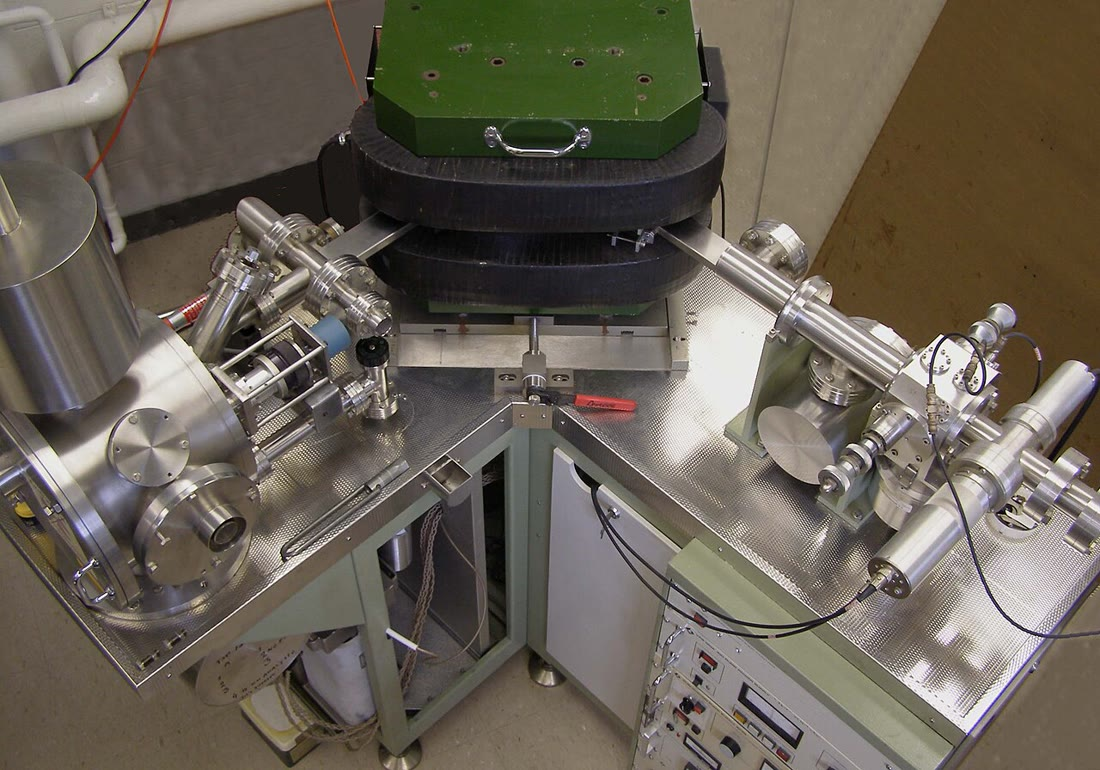
\includegraphics[width=0.42\linewidth]{images/book3/b1-tims.jpg}\hfill
\begin{minipage}[b]{0.55\linewidth}
Um espectrômetro de massa de ionização térmica (à esquerda) mede as razões isotópicas de
elementos como o estrôncio. O elemento, separado da amostra dissolvida por química, é carregado
em um filamento metálico em vácuo; aquecido, ele libera íons, que são acelerados e desviados pelo
campo do grande eletroímã (as bobinas pretas no centro), os íons mais leves mais que os mais
pesados, de modo que cada isótopo atinge seu próprio coletor. Razões entre isótopos são o que o
instrumento mede melhor, e por isso os métodos construídos só sobre razões são os mais precisos.
(Fotografia: Radiogenic, CC0, via Wikimedia Commons.)
\end{minipage}
\end{inthelab}
% ledger: commons:tims, amherst:constants

\section{Potássio--argônio, urânio--chumbo e radiocarbono}\label{sec:b1:radiometric-methods:kar}

\subsection*{Um pai com duas filhas}

\begin{definition}[Decaimento ramificado]\label{def:b1:radiometric-methods:branching}
Um pai sofre \emph{decaimento ramificado}\index{decaimento ramificado} quando seus núcleos
decaem por dois ou mais caminhos para filhas diferentes. Cada caminho $i$ tem sua própria
constante parcial de decaimento $\lambda_i$; o pai decai com a constante total
$\lambda = \sum_i \lambda_i$, e uma fração $\lambda_i/\lambda$ dos decaimentos segue o
caminho~$i$. O potássio-40 decai para cálcio-40 com $\lambda_\beta =
\num{4.962e-10}$ por ano e para argônio-40 com $\lambda_e = \num{0.581e-10}$ por
ano.
\end{definition}
% ledger: amherst:constants, iaea:k40-branches

\begin{proposition}[A idade potássio--argônio]\label{prop:b1:radiometric-methods:kar}
Um \omterm{def:b1:rock-forming-minerals:mineral}{mineral} que reteve todo o argônio nele produzido, e não continha nenhum quando se formou,
contém após um tempo $t$
\[
  {}^{40}\mathrm{Ar}^* = \frac{\lambda_e}{\lambda}\;{}^{40}\mathrm{K}\,\bigl(e^{\lambda t} - 1\bigr),
  \qquad\text{logo}\qquad
  t = \frac{1}{\lambda}\,\ln\!\left(1 + \frac{\lambda}{\lambda_e}\,
      \frac{{}^{40}\mathrm{Ar}^*}{{}^{40}\mathrm{K}}\right),
\]
em que ${}^{40}\mathrm{K}$ é o número de átomos de potássio-40 hoje e $\lambda =
\lambda_\beta + \lambda_e$.
\end{proposition}

\begin{proof}
O pai decai com a constante total $\lambda$, qualquer que seja o caminho, então pela
\cref{prop:b1:radiometric-methods:growth} o número de decaimentos no tempo $t$ é
${}^{40}\mathrm{K}\,(e^{\lambda t} - 1)$. Cada decaimento segue o caminho do argônio com
probabilidade $\lambda_e/\lambda$, independentemente dos outros; no número muito grande de
decaimentos, a fração que deu argônio é $\lambda_e/\lambda$. Isso dá ${}^{40}\mathrm{Ar}^*$;
resolvendo para $t$ obtém-se a idade.
\end{proof}

O expoente guarda a constante total e o fator à frente a parcial: usar $\lambda_e$ no expoente,
como se o argônio fosse o único caminho, daria uma idade totalmente errada. O ramo do cálcio
carrega nove décimos dos decaimentos, mas é inútil para datar, porque o cálcio-40 é o isótopo
comum de um elemento abundante nas rochas; o argônio, um gás nobre, escapa de um magma, de modo
que um cristal começa com quase nenhum. O potássio-40 é \qty{0.0117}{\percent} dos átomos de
potássio. O método precisa das quantidades absolutas de potássio e de argônio, medidas
separadamente. Argônio do ar, presente em toda rocha, é reconhecido por seu argônio-36 e
subtraído com a razão atmosférica $^{40}\mathrm{Ar}/^{36}\mathrm{Ar} = 295.5$.
% ledger: tulane:kar, iaea:k40-branches, amherst:constants, nmgrl:kar

O método falha de duas maneiras. Argônio em excesso torna as idades velhas demais: uma lava que
esfria depressa pode aprisionar argônio do \omterm{def:b1:layered-earth:layers}{manto} em bolhas, e lavas históricas costumam dar
idades potássio--argônio de 1 a 2 milhões de anos, um erro que só importa para rochas jovens. A
perda de argônio as torna jovens demais: a maioria dos \omterm{def:b1:rock-forming-minerals:mineral}{minerais} perde argônio quando aquecidos
acima de cerca de \qty{300}{\celsius}, de modo que um metamorfismo posterior zera o relógio
total ou parcialmente, e uma perda parcial dá uma idade entre os dois eventos que não data
nenhum deles. \omterm{def:b1:rock-forming-minerals:mineral}{Minerais} ricos em potássio são preferidos: sanidina e biotita, depois \omterm{def:b1:rock-forming-minerals:groups}{plagioclásio}
ou hornblenda.
% ledger: tulane:kar, nmgrl:kar

O método argônio--argônio mede apenas razões. A amostra é irradiada com nêutrons rápidos no
núcleo de um reator nuclear, ao lado de um \omterm{def:b1:rock-forming-minerals:mineral}{mineral} padrão de idade conhecida; a reação
transforma parte de seu potássio-39 em argônio-39, que então representa o potássio, e o padrão
dá o rendimento da reação. Os dois isótopos são medidos juntos no mesmo gás. A amostra pode
então ser aquecida em etapas, com um forno ou um laser; cada etapa dá uma idade, e as idades
são plotadas contra a fração acumulada de argônio-39 liberada, um espectro de idades. Etapas que
concordam dentro de seus erros formam um patamar; um espectro sem um patamar alerta que o
\omterm{def:b1:rock-forming-minerals:mineral}{mineral} não permaneceu fechado. A sincronia do impacto e da extinção no fim do Cretáceo repousa
sobre idades argônio--argônio.
% ledger: amherst:arar, nmgrl:arar, renne:kpg

\subsection*{Dois relógios de urânio}

O urânio tem dois isótopos de vida longa, o urânio-238 decaindo para chumbo-206 e o urânio-235
para chumbo-207, em taxas diferentes; hoje $^{235}\mathrm{U}/^{238}\mathrm{U} = 0.0072567$, um
átomo em 137.8. Um \omterm{def:b1:rock-forming-minerals:mineral}{mineral} que contém urânio carrega assim dois relógios independentes, cada um
com sua própria equação de crescimento, ${}^{206}\mathrm{Pb}^* = {}^{238}\mathrm{U}\,(e^{\lambda_{238} t} - 1)$
e ${}^{207}\mathrm{Pb}^* = {}^{235}\mathrm{U}\,(e^{\lambda_{235} t} - 1)$. Se as duas idades
concordam, diz-se que são concordantes, e a concordância é um teste de que o \omterm{def:b1:rock-forming-minerals:mineral}{mineral} permaneceu
fechado, algo que nenhum relógio isolado pode fornecer. A \omterm{def:b1:cross-sections:unconformity}{discordância} vem sobretudo do chumbo
perdido de partes do cristal danificadas pela radiação do próprio urânio; um gráfico das duas
razões uma contra a outra, o diagrama de concórdia, recupera então tanto a idade do cristal
quanto a do evento que o fez perder chumbo --- uma ferramenta do Livro~5.
% ledger: amherst:constants, tulane:upb-zircon

O zircão, $\mathrm{ZrSiO_4}$, é o \omterm{def:b1:rock-forming-minerals:mineral}{mineral} de escolha: incorpora urânio em sua estrutura, mas
quase nenhum chumbo, de modo que quase todo o seu chumbo é radiogênico; é duro, resiste ao
intemperismo e sobrevive ao metamorfismo, de modo que grãos erodidos de uma rocha mantêm sua
idade nas areias derivadas dela. Apatita e esfeno também são usados, com menos frequência.
% ledger: tulane:upb-zircon, commons:zircon-cl

\subsection*{Radiocarbono}

O carbono-14 é produzido continuamente na alta atmosfera a partir do nitrogênio-14 atingido por
raios cósmicos. Ele se une ao carbono da atmosfera; organismos vivos trocam carbono com a
atmosfera e mantêm sua proporção de carbono-14. Na morte a troca para e o carbono-14 decai de
volta a nitrogênio-14. Como a proporção inicial é a da atmosfera, a idade segue da lei de
decaimento sozinha, sem \omterm{def:b1:radiometric-methods:isochron}{isócrona}: $t = -\tau \ln(A/A_0)$, em que $A$ é a atividade do carbono da
amostra, $A_0$ a do carbono vivo e $\tau =
1/\lambda$ a vida média. Madeira, carvão, osso, dente e concha são datados desse modo, até
algumas dezenas de milhares de anos: cerca de \num{70000} anos no máximo.
% ledger: tulane:c14, iaea:c14

\begin{definition}[Idade radiocarbono, curva de calibração]\label{def:b1:radiometric-methods:radiocarbon}
A \emph{idade radiocarbono}\index{idade radiocarbono} (convencional) de uma amostra é
\[
  t = -8033 \,\ln \frac{A_{\mathrm{SN}}}{A_{\mathrm{ON}}} \ \text{anos AP},
\]
onde $A_{\mathrm{SN}}$ é a atividade do carbono da amostra e $A_{\mathrm{ON}}$ a do padrão de
referência; usa a meia-vida de \num{5568} anos (vida média \num{8033} anos), normaliza as
atividades para o fracionamento isotópico do carbono ($\delta^{13}\mathrm{C} = \qty{-25}{\permil}$),
e conta os anos antes de 1950 d.C. (BP, ``antes do presente''). Uma \emph{curva de
calibração}\index{curva de calibração} dá a idade radiocarbono de amostras de idade civil
conhecida; lida ao contrário, ela converte uma idade radiocarbono em uma faixa de idades civis
(cal BP).
\end{definition}
% ledger: sp77:conventional-age, reimer20:intcal20

A \omterm{def:b1:radiometric-methods:radiocarbon}{idade radiocarbono} não é uma idade em anos civis, por duas razões. A meia-vida de \num{5568}
anos, o valor de Libby, mantido por convenção, é menor que os \num{5700} anos verdadeiros, de
modo que as \omterm{def:b1:radiometric-methods:radiocarbon}{idades radiocarbono} ficam cerca de \qty{2.4}{\percent} curtas. Mais importante, a
proporção de carbono-14 na atmosfera não foi constante. A \omterm{def:b1:radiometric-methods:radiocarbon}{curva de calibração} mede os dois
efeitos juntos, em arquivos datados de modo independente: anéis de árvores até cerca de
\num{13900} cal BP, e além, sequências flutuantes de anéis de árvores, sedimentos de lagos e de
mar, depósitos de cavernas e corais, até \num{55000} cal BP (figura abaixo).
% ledger: sp77:conventional-age, iaea:c14, reimer20:intcal20

\begin{omfigure}
\begin{tikzpicture}
\begin{axis}[name=main, omrecord, width=0.5\linewidth, height=6cm, xmin=0, xmax=12, ymin=0, ymax=12,
  xlabel={idade civil (mil cal BP)}, ylabel={idade radiocarbono (mil BP)},
  xtick={0,2,...,12}, ytick={0,2,...,12}]
% figdata/bachelor-1/radiocarbon.py, IntCal20 (dataset bachelor-1-intcal20); ledger: data:b3-intcal20
\addplot[black!50, dashed, domain=0:12, samples=2] {x};
\addplot[omDef, line width=0.9pt] table[x=cal, y=c14] {figdata/out/bachelor-1-radiocarbon-curve.dat};
\draw[omThm, line width=0.6pt] (axis cs:2.3,2.3) rectangle (axis cs:2.9,2.9);
\node[font=\scriptsize, anchor=east, text=black!60] at (axis cs:8.4,10.4) {idades iguais};
\node[font=\scriptsize, text=omDef, anchor=north west] at (axis cs:7.4,5.6) {IntCal20};
\end{axis}
\begin{axis}[at={(main.east)}, anchor=west, xshift=2.1cm, omrecord, width=0.38\linewidth, height=6cm,
  xmin=2300, xmax=2900, ymin=2300, ymax=2900, xlabel={idade civil (cal BP)}, ylabel={idade radiocarbono (BP)},
  xtick={2300,2500,2700,2900}, ytick={2300,2500,2700,2900},
  x tick label style={/pgf/number format/.cd, set thousands separator={}},
  y tick label style={/pgf/number format/.cd, set thousands separator={}}]
\addplot[name path=hi, draw=none, forget plot] table[x=cal, y=hi] {figdata/out/bachelor-1-radiocarbon-zoom.dat};
\addplot[name path=lo, draw=none, forget plot] table[x=cal, y=lo] {figdata/out/bachelor-1-radiocarbon-zoom.dat};
\addplot[omDef!25, forget plot] fill between[of=hi and lo];
\addplot[omDef, line width=0.8pt] table[x=cal, y=c14] {figdata/out/bachelor-1-radiocarbon-zoom.dat};
\addplot[omThm, line width=0.6pt, domain=2300:2900, samples=2] {2480};
\draw[omThm, densely dotted] (axis cs:2495,2300) -- (axis cs:2495,2480);
\draw[omThm, densely dotted] (axis cs:2699,2300) -- (axis cs:2699,2480);
\node[font=\scriptsize, text=omThm, anchor=south west] at (axis cs:2310,2485) {$2480$ BP};
\end{axis}
\end{tikzpicture}

{\small À esquerda: a \omterm{def:b1:radiometric-methods:radiocarbon}{curva de calibração} IntCal20 sobre os últimos \num{12000} anos, \omterm{def:b1:radiometric-methods:radiocarbon}{idade
radiocarbono} contra idade civil; a linha tracejada é onde as duas seriam iguais. À direita: a
caixa à esquerda ampliada, com a faixa de uma incerteza padrão da curva. Entre \num{2500} e
\num{2700} cal BP a curva é quase plana: uma \omterm{def:b1:radiometric-methods:radiocarbon}{idade radiocarbono} de 2480 anos BP corresponde a
idades civis de cerca de \num{2495} a \num{2699} cal BP.}
\label{fig:b1:radiometric-methods:intcal}
\end{omfigure}
% ledger: data:b3-intcal20, reimer20:intcal20

Em \num{2000} cal BP a curva dá \num[uncertainty-mode=separate]{2070 \pm 14} anos BP; em
\num{12000} cal BP, \num{10306}: \omterm{def:b1:radiometric-methods:radiocarbon}{idades radiocarbono} ali são \num{1694} anos mais jovens que as
idades civis, muito mais que os \qty{2.4}{\percent} da meia-vida. A curva oscila, e onde é plana
uma \omterm{def:b1:radiometric-methods:radiocarbon}{idade radiocarbono} corresponde a uma longa faixa de idades civis, por mais precisa que seja a
medida.
% ledger: data:b3-intcal20

\begin{dated}{2020}
% ledger: reimer20:intcal20
A curva em uso para o Hemisfério Norte é a IntCal20, publicada em 2020. Ela substituiu a
IntCal13, acrescentando novos dados e estendendo a curva a \num{55000} cal BP, com curvas
separadas para o Hemisfério Sul e para a superfície do oceano. \omterm{def:b1:radiometric-methods:radiocarbon}{Curvas de calibração} são revisadas
à medida que novos arquivos são medidos, de modo que uma idade civil deve nomear a curva que a
produziu.
\end{dated}

\section{Temperatura de fechamento}\label{sec:b1:radiometric-methods:closure}

Um \omterm{def:b1:rock-forming-minerals:mineral}{mineral} que cristaliza a partir de um magma a \qty{800}{\celsius} não inicia seu relógio de
imediato. Enquanto está quente, átomos da filha --- o argônio sobretudo --- difundem-se por sua
rede e escapam; só quando esfriou o bastante a difusão torna-se lenta demais para importar, e a
filha começa a se acumular.
% ledger: leeds:closure, tulane:kar, tulane:magma-types

\begin{definition}[Temperatura de fechamento, idade de resfriamento]\label{def:b1:radiometric-methods:closure}
A \emph{temperatura de fechamento}\index{temperatura de fechamento} de um \omterm{def:b1:rock-forming-minerals:mineral}{mineral} para um sistema
de decaimento é a temperatura abaixo da qual os átomos-pai e filha não entram nem saem de sua
rede depressa o bastante para importar, de modo que o \omterm{def:b1:rock-forming-minerals:mineral}{mineral} se comporta como um sistema
fechado. Uma \emph{idade de resfriamento}\index{idade de resfriamento} é uma idade medida em um
\omterm{def:b1:rock-forming-minerals:mineral}{mineral} que se formou acima de sua temperatura de fechamento: ela data o momento em que o \omterm{def:b1:rock-forming-minerals:mineral}{mineral}
resfriou através dessa temperatura, não o momento em que se formou.
\end{definition}
% ledger: leeds:closure

As \omterm{def:b1:radiometric-methods:closure}{temperaturas de fechamento} diferem de \omterm{def:b1:rock-forming-minerals:mineral}{mineral} para \omterm{def:b1:rock-forming-minerals:mineral}{mineral}, porque as redes diferem, e de
elemento para elemento, porque átomos diferentes se difundem por uma mesma rede em taxas
diferentes (figura abaixo). São aproximadas: duas tabelas dão \qty{280}{\celsius} e
\qty{350}{\celsius} para o argônio na biotita, \qty{530}{\celsius} e \qty{550}{\celsius} para o
argônio na hornblenda. Traços de fissão, as trilhas de dano deixadas em um cristal pela fissão
espontânea de núcleos de urânio, se curam a temperaturas ainda mais baixas.
% ledger: leeds:closure, amherst:closure

\begin{omfigure}
\begin{tikzpicture}
\begin{axis}[width=0.8\linewidth, height=7cm, xbar, bar width=7pt, xmin=0, xmax=850,
  xlabel={temperatura de fechamento (\unit{\celsius})},
  symbolic y coords={zrupb,spupb,hbar,mssr,msar,btsr,btar,zrft,kfsar,apft},
  ytick={zrupb,spupb,hbar,mssr,msar,btsr,btar,zrft,kfsar,apft}, y dir=reverse, enlarge y limits=0.07,
  yticklabels={{zircão, U--Pb},{esfeno, U--Pb},{hornblenda, K--Ar},{muscovita, Rb--Sr},{muscovita, K--Ar},{biotita, Rb--Sr},{biotita, K--Ar},{zircão, traços de fissão},{feldspato-K, K--Ar},{apatita, traços de fissão}},
  y tick label style={font=\scriptsize}, x tick label style={font=\scriptsize},
  axis x line*=bottom, axis y line*=left]
% ledger: leeds:closure (values as tabulated; > lower bound, ~ approximate, ranges and +- as given)
\addplot[fill=omDef!55, draw=omDef, error bars/.cd, x dir=both, x explicit]
  coordinates {(750,zrupb) (650,spupb) (530,hbar) +- (40,0) (500,mssr) (350,msar) (320,btsr)
               (280,btar) +- (40,0) (200,zrft) +- (25,0) (130,kfsar) (105,apft) +- (10,0)};
\node[font=\scriptsize, anchor=west] at (axis cs:755,zrupb) {$> 750$};
\node[font=\scriptsize, anchor=west] at (axis cs:655,spupb) {$> 650$};
\node[font=\scriptsize, anchor=west] at (axis cs:575,hbar) {$530 \pm 40$};
\node[font=\scriptsize, anchor=west] at (axis cs:505,mssr) {$500$};
\node[font=\scriptsize, anchor=west] at (axis cs:355,msar) {$\approx 350$};
\node[font=\scriptsize, anchor=west] at (axis cs:325,btsr) {$320$};
\node[font=\scriptsize, anchor=west] at (axis cs:325,btar) {$280 \pm 40$};
\node[font=\scriptsize, anchor=west] at (axis cs:230,zrft) {$175$--$225$};
\node[font=\scriptsize, anchor=west] at (axis cs:135,kfsar) {$\approx 130$, com fuga};
\node[font=\scriptsize, anchor=west] at (axis cs:120,apft) {$105 \pm 10$};
\end{axis}
\end{tikzpicture}

{\small \omterm{def:b1:radiometric-methods:closure}{Temperaturas de fechamento} dos principais relógios \omterm{def:b1:rock-forming-minerals:mineral}{minerais}, a partir de uma tabela
publicada. U--Pb é urânio--chumbo, K--Ar potássio--argônio (e argônio--argônio), Rb--Sr
rubídio--estrôncio. Para os traços de fissão o valor é a temperatura em que os traços se curam.}
\label{fig:b1:radiometric-methods:closure}
\end{omfigure}

Em um plúton que esfriou devagar, os relógios fecham-se, portanto, um após o outro, do mais
quente ao mais frio: primeiro o zircão, perto de sua cristalização, depois a hornblenda, depois a
muscovita e a biotita. A dispersão de suas idades registra o resfriamento.

\begin{proposition}[Taxa de resfriamento entre dois fechamentos]\label{prop:b1:radiometric-methods:cooling}
Se dois \omterm{def:b1:rock-forming-minerals:mineral}{minerais} de uma mesma rocha, de \omterm{def:b1:radiometric-methods:closure}{temperaturas de fechamento} $T_1 > T_2$, dão as \omterm{def:b1:radiometric-methods:closure}{idades de
resfriamento} $t_1 > t_2$, a taxa média de resfriamento entre os dois fechamentos é
\[
  \dot T = \frac{T_1 - T_2}{t_1 - t_2}.
\]
Se a rocha estava a uma profundidade onde a temperatura subia com a profundidade, com gradiente
constante $G$ abaixo de uma superfície à temperatura $T_s$, ela estava à profundidade $z_i
= (T_i - T_s)/G$ quando o relógio $i$ fechou.
\end{proposition}

\begin{proof}
A rocha estava a $T_1$ no tempo $t_1$ e a $T_2$ no tempo $t_2$; a taxa média de variação de sua
temperatura é a razão das duas diferenças. Com um geoterma linear
(\cref{def:b1:heat-budget:geotherm}), $T = T_s + G z$, o que dá a profundidade.
\end{proof}

A profundidade dá uma taxa de exumação quando o tempo em que a rocha chegou à superfície é
conhecido --- como no problema deste capítulo. O método é grosseiro: as \omterm{def:b1:radiometric-methods:closure}{temperaturas de
fechamento} são incertas em dezenas de graus, e o geoterma é suposto constante no tempo. A
termocronologia, a reconstrução detalhada de trajetórias temperatura--tempo a partir de muitos
relógios, é assunto do Livro~5.

\section{Datação de sequências sedimentares}\label{sec:b1:radiometric-methods:sediments}

A maioria das rochas sedimentares não pode ser datada diretamente. Seus grãos são mais velhos
que a rocha: um zircão detrítico, como o grão do início deste capítulo, data a rocha de onde foi
erodido. O radiocarbono data apenas matéria orgânica jovem. As idades da escala vêm, portanto, de
rochas que cristalizaram no momento em que foram depositadas --- cinzas vulcânicas e derrames de
lava dentro da sequência --- e de rochas ígneas que a cortam.
% ledger: tulane:upb-zircon, tulane:c14, commons:zircon-cl

\begin{definition}[Idade de contenção]\label{def:b1:radiometric-methods:bracketing}
Uma \emph{idade de contenção}\index{idade de contenção} é um limite posto na idade de um nível
sedimentar por rochas datadas relacionadas a ele pelos princípios da estratigrafia: uma idade
máxima a partir de uma camada datada abaixo dele, ou a partir do grão detrítico mais jovem nele;
uma idade mínima a partir de uma camada datada acima dele, ou de uma intrusão que o corta. Um
nível entre um máximo e um mínimo fica contido.
\end{definition}

\begin{omfigure}
\begin{tikzpicture}[x=1cm, y=0.62cm]
  % column
  \fill[lith shale] (0,0) rectangle (2.4,3);
  \fill[lith sandstone] (0,3) rectangle (2.4,6);
  \fill[lith shale] (0,6) rectangle (2.4,9);
  \fill[lith limestone] (0,9) rectangle (2.4,12);
  \draw (0,0) rectangle (2.4,12);
  % ash bed below, lava flow above
  \fill[omThm!70] (0,2.0) rectangle (2.4,2.3);
  \fill[black!65] (0,9.0) rectangle (2.4,9.6);
  % boundary
  \draw[omDef, line width=1.2pt] (-0.3,7.2) -- (2.7,7.2);
  % dyke cutting everything
  \fill[black!40] (1.55,0) -- (1.85,0) -- (1.95,12) -- (1.65,12) -- cycle;
  % detrital zircons
  \foreach \p in {(0.4,3.6),(0.9,4.5),(0.5,5.4),(1.2,3.9),(0.8,5.0)}
    \fill[omThm] \p circle (1.3pt);
  % labels
  \node[anchor=west, font=\small, align=left] at (3.0,2.15) {camada de cinza, $t_1$: idade máxima};
  \node[anchor=west, font=\small, align=left] at (3.0,4.5) {zircão detrítico mais jovem, $t_0$:\\idade máxima do arenito};
  \node[anchor=west, font=\small, text=omDef] at (3.0,7.2) {nível a datar};
  \node[anchor=west, font=\small, align=left] at (3.0,9.3) {derrame de lava, $t_2$: idade mínima};
  \node[anchor=west, font=\small, align=left] at (3.0,11.3) {dique, $t_3$: idade mínima de\\cada camada que ele corta};
  \draw[black!50] (2.5,2.15) -- (2.95,2.15);
  \draw[black!50] (1.25,4.5) -- (2.95,4.5);
  \draw[black!50] (2.5,9.3) -- (2.95,9.3);
  \draw[black!50] (1.95,11.3) -- (2.95,11.3);
\end{tikzpicture}

{\small Idades que contêm um nível em uma sequência sedimentar (esquemático). A camada de cinza
abaixo e o zircão detrítico mais jovem do arenito dão idades máximas; o derrame de lava acima e o
dique que corta toda a sequência dão idades mínimas. O nível é mais jovem que $t_1$ e mais velho
que $t_2$; o dique acrescenta apenas que ele é mais velho que $t_3$.}
\label{fig:b1:radiometric-methods:bracketing}
\end{omfigure}

As melhores contenções são próximas e precisas: duas camadas de cinza a alguns metros de
distância, datadas em zircão com precisão de algumas dezenas de milhares de anos, com o nível
entre elas interpolado por \cref{prop:b1:stratigraphic-scale:interpolation}. Em Meishan, o GSSP
da base do Triássico fica entre cinco camadas de cinza datadas; a extinção é contida entre
\qty[uncertainty-mode=separate]{251.941(37)}{\Ma} e \qty[uncertainty-mode=separate]{251.880(31)}{\Ma},
e a base do \omterm{def:b1:stratigraphic-scale:chronostratigraphy}{sistema} é colocada em \qty[uncertainty-mode=separate]{251.902(24)}{\Ma}
(\cref{sec:b1:stratigraphic-scale:extinctions}). Camadas de cinza, carregadas pelo vento através
das fácies, são ao mesmo tempo linhas de tempo e relógios.
% ledger: burgess:end-permian, gssp:induan, ics:base.Triassic

A escala só é tão precisa quanto as camadas datadas perto de cada limite. A base do Triássico é
conhecida a \qty{0.024}{\Myr}, uma parte em dez mil; a base do Carbonífero a \qty{0.19}{\Myr}; a
base do Devoniano a \qty{1.36}{\Myr}. Onde nenhuma camada datada fica perto de um limite, sua
idade é interpolada entre outras distantes, e sua incerteza cresce em conformidade. Cada nova
camada de cinza datada perto de um limite pode deslocá-lo, por isso a carta traz uma data de
versão.
% ledger: ics:base.Triassic, ics:base.Carboniferous, gssp:lochkovian

\section{Exercícios}

\begin{exercise}[$\star$]\label{exo:b1:radiometric-methods:1}
(a)~Um \omterm{def:b1:rock-forming-minerals:mineral}{mineral} contém três vezes mais átomos de \omterm{def:b1:radiometric-methods:radiogenic}{filha radiogênica} que átomos de pai. Quantas
meias-vidas ele tem? (b)~Calcule $D^*/P$ após \qty{310}{\Myr} para o rubídio-87 e para o
urânio-235, com as constantes de \cref{tab:b1:radiometric-methods:systems}. Qual razão é mais
fácil de medir com precisão? (c)~Após quantas meias-vidas resta menos de \qty{1}{\percent} do
pai?
% ledger: villa22:rb87, amherst:constants
\end{exercise}

\begin{exercise}[$\star$]\label{exo:b1:radiometric-methods:2}
Qual método de \cref{tab:b1:radiometric-methods:systems} você usaria, e em qual material, para
datar: (a)~carvão de uma lareira de cerca de \num{8000} anos; (b)~uma camada de cinza que se
pensa ter cerca de \qty{66}{\Ma}, rica em sanidina e zircão; (c)~um granito de cerca de
\qty{2.7}{\Ga}; (d)~uma concha de cerca de \num{40000} anos; (e)~um calcário do Jurássico sem
nenhuma camada vulcânica?
% ledger: tulane:c14, tulane:kar, tulane:upb-zircon
\end{exercise}

\begin{exercise}[$\star$]\label{exo:b1:radiometric-methods:3}
O carbono de um pedaço de madeira tem um quarto da atividade do padrão, após normalização.
(a)~Calcule sua \omterm{def:b1:radiometric-methods:radiocarbon}{idade radiocarbono} convencional. (b)~Calcule sua idade com a meia-vida de
\num{5700} anos. (c)~Por que nenhuma dessas é sua idade em anos civis, e como essa idade é
obtida?
% ledger: sp77:conventional-age, iaea:c14
\end{exercise}

\begin{exercise}[$\star$]\label{exo:b1:radiometric-methods:4}
Um granito dá uma idade urânio--chumbo no zircão de \qty{420}{\Ma}, uma idade
potássio--argônio na hornblenda de \qty{410}{\Ma} e uma na biotita de \qty{398}{\Ma}. (a)~Por que
as três idades são diferentes, e nessa ordem? (b)~Com as \omterm{def:b1:radiometric-methods:closure}{temperaturas de fechamento} da figura de
\cref{sec:b1:radiometric-methods:closure}, calcule a taxa média de resfriamento entre
os fechamentos da hornblenda e da biotita. (c)~O que se pode dizer da taxa de resfriamento
entre o fechamento do zircão e o da hornblenda?
% ledger: leeds:closure
\end{exercise}

\begin{exercise}[$\star\star$]\label{exo:b1:radiometric-methods:5}
Quatro amostras de rocha total de um gnaisse (dados de exercício) dão
$^{87}\mathrm{Rb}/^{86}\mathrm{Sr} = 2.0$, $5.0$, $9.0$, $14.0$ e
$^{87}\mathrm{Sr}/^{86}\mathrm{Sr} = 0.7323$, $0.7741$, $0.8307$, $0.9010$.
(a)~Ajuste a reta dos mínimos quadrados pelo método de
\cref{met:b1:radiometric-methods:isochron}. (b)~Calcule a idade e a \omterm{def:b1:radiometric-methods:isochron}{razão inicial}. (c)~Calcule
$s$ e a incerteza da idade. (d)~A \omterm{def:b1:radiometric-methods:isochron}{razão inicial} aponta para uma fonte no \omterm{def:b1:layered-earth:layers}{manto} ou na \omterm{def:b1:layered-earth:layers}{crosta}?
% ledger: villa22:rb87, tulane:sr-initial
\end{exercise}

\begin{exercise}[$\star\star$]\label{exo:b1:radiometric-methods:6}
Uma sanidina de uma camada de cinza contém \qty{10.0}{\percent} de potássio em massa e
\qty{1.169}{nmol} de argônio-40 radiogênico por grama. (a)~Com a massa atômica do potássio,
\qty{39.098}{g.mol^{-1}}, e a abundância do potássio-40, calcule o número de mols de
potássio-40 por grama. (b)~Calcule a idade potássio--argônio. (c)~Se \qty{0.5}{\percent} do
argônio medido tivesse sido aprisionado quando a cinza caiu, em quanto a idade estaria velha
demais? Isso é uma preocupação aqui?
% ledger: ciaaw:K, iaea:k40-branches, amherst:constants, tulane:kar
\end{exercise}

\begin{exercise}[$\star\star$]\label{exo:b1:radiometric-methods:7}
A curva IntCal20 dá as \omterm{def:b1:radiometric-methods:radiocarbon}{idades radiocarbono} \num[uncertainty-mode=separate]{2070 \pm 14} anos BP a
\num{2000} cal BP, \num{7178} a \num{8000} cal BP e \num{10306} a \num{12000} cal BP.
(a)~Uma semente dá \num[uncertainty-mode=separate]{2070 \pm 14} anos BP. Qual é sua idade
civil? (b)~Outra dá \num[uncertainty-mode=separate]{2480 \pm 15} anos BP; com o painel da
direita da figura de \cref{sec:b1:radiometric-methods:kar}, dê sua faixa de idades civis e
explique por que ela é tão larga. (c)~Em quantos anos, e em que direção, as \omterm{def:b1:radiometric-methods:radiocarbon}{idades radiocarbono}
diferem das idades civis a \num{2000}, \num{8000} e \num{12000} cal BP? A diferença cresce em
proporção à idade?
% ledger: data:b3-intcal20
\end{exercise}

\begin{exercise}[$\star\star$]\label{exo:b1:radiometric-methods:8}
Em uma seção marinha, uma camada de cinza a \qty{4}{m} é datada de
\qty[uncertainty-mode=separate]{94.50(10)}{\Ma} e um derrame de lava a \qty{20}{m} de
\qty[uncertainty-mode=separate]{93.80(12)}{\Ma}; um dique que corta toda a seção é datado de
\qty[uncertainty-mode=separate]{93.20(8)}{\Ma}. O zircão detrítico mais jovem de um arenito a
\qtyrange{6}{10}{m} é de \qty[uncertainty-mode=separate]{95.3(4)}{\Ma}. Um limite de \omterm{def:b1:stratigraphic-scale:chronostratigraphy}{andar} é
posto a \qty{12}{m}. (a)~Quais das quatro idades contêm o limite, e quais não servem para ele?
(b)~Interpole sua idade e sua incerteza com
\cref{prop:b1:stratigraphic-scale:interpolation}. (c)~O que o zircão detrítico diz sobre o
arenito?
\end{exercise}

\begin{exercise}[$\star\star$]\label{exo:b1:radiometric-methods:9}
Dois zircões de um mesmo granito dão
$^{206}\mathrm{Pb}^*/^{238}\mathrm{U} = 0.08401$ e
$^{207}\mathrm{Pb}^*/^{235}\mathrm{U} = 0.6688$ (grão~A), e $0.05881$ e
$0.4682$ (grão~B). (a)~Calcule as duas idades de cada grão. (b)~Qual grão é concordante?
(c)~O grão~B perdeu parte de seu chumbo recentemente. Mostre que suas duas razões são
\qty{70}{\percent} das do grão~A, e explique por que suas duas idades diferem embora a perda
tenha sido a mesma para os dois isótopos.
% ledger: amherst:constants, tulane:upb-zircon
\end{exercise}

\begin{exercise}[$\star\star\star$]\label{exo:b1:radiometric-methods:10}
(a)~Mostre que quando $\lambda t \ll 1$ a equação da idade se reduz a $t \approx
(D^*/P)/\lambda$, e que o erro relativo dessa aproximação é próximo de
$\lambda t/2$. (b)~Calcule o erro para o rubídio-87 a \qty{310}{\Ma}, para o potássio-40 a
\qty{296}{\Ma} e para o urânio-238 a \qty{4.4}{\Ga}. (c)~Se $D^*/P$ for medido a
\qty{0.1}{\percent}, qual é a incerteza de uma idade rubídio--estrôncio de \qty{310}{\Ma}?
% ledger: villa22:rb87, amherst:constants
\end{exercise}

\begin{exercise}[$\star\star\star$]\label{exo:b1:radiometric-methods:11}
Uma biotita cristalizou e fechou-se há \qty{400}{\Myr}. Há \qty{200}{\Myr} um aquecimento breve
fez com que ela perdesse uma fração $f$ de seu argônio, após o que ela se fechou de novo.
(a)~Mostre que hoje
\[
  \frac{\lambda}{\lambda_e}\,\frac{^{40}\mathrm{Ar}^*}{^{40}\mathrm{K}} =
  (1 - f)\bigl(e^{\lambda t_1} - e^{\lambda t_2}\bigr) + e^{\lambda t_2} - 1,
\]
com $t_1 = \qty{400}{\Myr}$ e $t_2 = \qty{200}{\Myr}$. (b)~Calcule a idade potássio--argônio
aparente para $f = 0$, $0.3$, $0.6$ e $1$. (c)~Por que uma única idade potássio--argônio não pode
distinguir uma perda parcial de um evento mais jovem?
% ledger: amherst:constants, tulane:kar
\end{exercise}

\begin{exercise}[$\star\star\star$]\label{exo:b1:radiometric-methods:12}
Em \num{12000} cal BP a curva IntCal20 dá uma \omterm{def:b1:radiometric-methods:radiocarbon}{idade radiocarbono} de \num{10306} anos BP. (a)~Recalcule
a idade a partir da mesma razão de atividades com a meia-vida de \num{5700} anos. (b)~Quanto dos
\num{1694} anos pelos quais a \omterm{def:b1:radiometric-methods:radiocarbon}{idade radiocarbono} fica aquém da idade civil a convenção da
meia-vida explica? (c)~Supondo que o resto venha de uma proporção mais alta de carbono-14 na
atmosfera há \num{12000} anos, calcule em quanto, em por cento, ela excedeu a proporção do padrão.
% ledger: data:b3-intcal20, sp77:conventional-age, iaea:c14
\end{exercise}

\section{Problema: datando o granito de Varden e sua cobertura}

\begin{problem}[{Problema de fim de semana --- como quatro relógios datam a cristalização, o
resfriamento e o desmantelamento de um granito}]
\label{pb:b1:radiometric-methods:1}
% values: calc/ch25.py; the analyses are invented, consistent with the Varden granite of 310 Ma (region.py)
O granito das Colinas de Varden, a região inventada da série, intrude o embasamento xistoso e é
recoberto, acima de uma \omterm{def:b1:cross-sections:unconformity}{discordância}, pelo arenito triássico. Use as constantes de
\cref{tab:b1:radiometric-methods:systems}, as \omterm{def:b1:radiometric-methods:closure}{temperaturas de fechamento} da figura de
\cref{sec:b1:radiometric-methods:closure}, a massa atômica do potássio \qty{39.098}{g.mol^{-1}} e
a abundância do potássio-40, \qty{0.0117}{\percent} dos átomos de potássio. Todas as análises são
dados de exercício.

\medskip
\noindent\textbf{Parte I --- Uma isócrona de rocha total.} Seis amostras de rocha total dão:
\begin{center}
\small
\begin{tabular}{|l|cccccc|}
\hline
$^{87}\mathrm{Rb}/^{86}\mathrm{Sr}$ & 0.92 & 2.15 & 3.40 & 5.05 & 7.60 & 10.30 \\
$^{87}\mathrm{Sr}/^{86}\mathrm{Sr}$ & 0.71211 & 0.71718 & 0.72284 & 0.72986 & 0.74113 & 0.75261 \\
\hline
\end{tabular}
\end{center}
\begin{enumerate}
  \item Plote as seis amostras. Elas se alinham em uma reta?
  \item Calcule $\bar x$, $\bar y$, $S_{xx}$ e $S_{xy}$, depois a
        inclinação dos mínimos quadrados.
  \item Calcule a interseção. O que ela representa?
  \item Calcule a idade do granito.
  \item Calcule os resíduos, $s$, e a incerteza da idade.
  \item A \omterm{def:b1:radiometric-methods:isochron}{razão inicial} é mais próxima à do \omterm{def:b1:layered-earth:layers}{manto} ou à da \omterm{def:b1:layered-earth:layers}{crosta} continental? Se o magma fosse
        uma mistura de fusões com $0.7025$ e $0.710$, igualmente ricas em estrôncio, que parcela
        de seu estrôncio veio da \omterm{def:b1:layered-earth:layers}{crosta}?
\end{enumerate}

\noindent\textbf{Parte II --- Potássio e argônio.} Uma biotita contém
\qty{7.40}{\percent} de potássio em massa e \qty{4.139}{nmol} de argônio-40 radiogênico por
grama; uma hornblenda \qty{1.10}{\percent} e \qty{0.6333}{nmol.g^{-1}}.
\begin{enumerate}[resume]
  \item Calcule o número de átomos de potássio-40 em um grama da biotita.
  \item Calcule a idade potássio--argônio da biotita.
  \item Calcule a da hornblenda.
  \item Que idade a biotita daria se a ramificação fosse esquecida e todos os decaimentos fossem
        contados como argônio? Por que não se usa o cálcio-40 no lugar?
  \item Por que o excesso de argônio, aprisionado quando os \omterm{def:b1:rock-forming-minerals:mineral}{minerais} se formaram, pouco preocupa
        aqui?
  \item Ambas as idades são mais jovens que a idade da \omterm{def:b1:radiometric-methods:isochron}{isócrona}. Dê duas explicações, e diga
        como um espectro de idades argônio--argônio poderia distingui-las.
\end{enumerate}

\noindent\textbf{Parte III --- Resfriamento.} Um zircão do granito dá
$^{206}\mathrm{Pb}^*/^{238}\mathrm{U} = 0.049361$ e
$^{207}\mathrm{Pb}^*/^{235}\mathrm{U} = 0.35784$.
\begin{enumerate}[resume]
  \item Calcule as duas idades urânio--chumbo. São concordantes?
  \item Atribua a cada idade das Partes I a III o evento que ela data. Desenhe a temperatura do
        granito contra o tempo desde o zircão até a biotita.
  \item Calcule a taxa média de resfriamento entre os fechamentos da hornblenda e da biotita.
  \item O que se pode dizer da taxa de resfriamento entre o fechamento do zircão e o da
        hornblenda?
  \item Com uma incerteza de \qty{40}{\celsius} em cada uma das duas \omterm{def:b1:radiometric-methods:closure}{temperaturas de fechamento},
        independentes, que faixa de taxas de resfriamento é possível?
  \item Com a outra tabela citada no capítulo (\qty{550}{\celsius} para a hornblenda,
        \qty{350}{\celsius} para a biotita), que taxa se encontra? O que isso diz do resultado?
  \item Suponha um geoterma de \qty{30}{\celsius.km^{-1}} abaixo de uma superfície a
        \qty{10}{\celsius}. A que profundidade estava o granito quando a biotita fechou?
\end{enumerate}

\noindent\textbf{Parte IV --- A discordância.} Uma camada de cinza a \qty{18}{m} acima da base do
arenito triássico contém zircões com $^{206}\mathrm{Pb}^*/^{238}\mathrm{U} = 0.039108$ e
$^{207}\mathrm{Pb}^*/^{235}\mathrm{U} = 0.27577$. Uma segunda camada de cinza, a \qty{58}{m}
acima da base, é datada de \qty{245.30}{\Ma}. Zircões detríticos no metro mais baixo do arenito
dão idades em torno de \qty{310}{\Ma}.
\begin{enumerate}[resume]
  \item Calcule a idade da camada de cinza inferior.
  \item De onde vêm os zircões detríticos, e o que dizem sobre a idade do arenito?
  \item Calcule a taxa de acumulação do arenito entre as camadas de cinza, e a idade de sua base,
        supondo a mesma taxa abaixo da cinza inferior.
  \item Qual é a duração da lacuna do registro na \omterm{def:b1:cross-sections:unconformity}{discordância}, da cristalização do granito à
        deposição do arenito?
  \item Calcule a taxa média de erosão que trouxe o granito da profundidade da questão~19 à
        superfície. Que suposição isso faz sobre onde o granito erodido estava?
  \item Qual é a taxa de resfriamento do granito?
\end{enumerate}
\end{problem}
